\documentclass[a4paper,12pt]{article}
\usepackage[utf8]{inputenc}
\usepackage{graphicx}
\usepackage{amsmath}
\usepackage{hyperref}
\usepackage{enumitem}
\usepackage{geometry}
\usepackage{fancyhdr}
\usepackage{titlesec}
\usepackage{tabularx}

% Page Layout
\geometry{margin=1in}
\pagestyle{fancy}
\fancyhf{}
\fancyhead[L]{\textbf{Relatório do Projeto}}
\fancyhead[R]{\thepage}

% Title Formatting
\titleformat{\section}{\Large\bfseries}{\thesection}{1em}{}
\titleformat{\subsection}{\large\bfseries}{\thesubsection}{1em}{}

% Title Page
\title{Relatório do Projeto: 1ª Versão}
%\author{Your Name \\ Your Institution \\ \texttt{your.email@example.com}}
\date{\today}

% Page layout settings
\geometry{top=1in, bottom=1in, left=1.25in, right=1in}

% No header or footer on title page
\pagestyle{empty}

\begin{document}

% Title Page
\begin{center}
    \large\textbf{UNIVERSIDADE DE AVEIRO} \\[1.5cm]
    
    
\includegraphics[width=10cm]{images/Universidade-de-Aveiro.png} \\[1.5cm]
    
    \Huge \textbf{Técnicas de Mineração\\ de Texto - 2} \\[1.5cm]

    % Isto fica podre
    %\Large \textbf{Gabriel Boia} \\[0.5cm]
    %\Large \textbf{Guilherme Matos} \\[0.5cm]
    %\Large \textbf{Rafael Dias} \\[0.5cm]
    %\Large \textbf{Tiago Costa} \\[0.5cm]
    %\Large \textbf{Tiago Almeida} \\[2cm]

    % Incluir imagem relacionada com o trabalho
    % 
\includegraphics[width=5cm]{images/Universidade-de-Aveiro.png} \\[2cm]
    
    \normalsize Licenciatura em Engenharia de Computadores e Informatica \\[0.5cm]
    UC: Projeto em Engenharia de Computadores e Informática \\[0.5cm]
    Equipa: Gabriel Boia (113167), Guilherme Matos (114252), Rafael Dias (114258), Tiago Costa (114629) e Tiago Almeida (113106) \\[0.5cm]
    Supervisor: Luís Filipe de Seabra Lopes \\[2cm]
    \vfill
    \textbf{\today} \\[1cm]
\end{center}
\newpage

% Resumo
% \clearpage
% \thispagestyle{empty} % No header or footer

% \begin{center}
%     \Huge \textbf{Resumo} \\[1.5cm]
% \end{center}

% \noindent
% bla bla bla...

% Resto to relatório
\newpage
\maketitle
\tableofcontents
\newpage

\section{Introdução}
Quando empresas trabalham com grandes quantidades de dados, é importante que os mesmos sigam um padrão definido, para que a procura e atualização de informação dentro de conjuntos de dados seja rápida e eficaz. O grupo responsável pelo projeto aqui descrito propôs-se, então, a procurar resolver este problema através de um método automático de correção de bases de dados. Os dados de treino utilizados foram fornecidos pela empresa que submeteu a proposta do projeto: Administração dos Portos de Sines e do Algarve, S.A.
\\
Posto isto, o presente relatório tem como objetivo dar a conhecer o trabalho realizado neste âmbito, inserido na Unidade Curricular de "Projeto em Engenharia de Computadores e Informática". Este trabalho foi realizado ao longo do ano letivo 2024/2025, sob supervisão do professor Luís Seabra Lopes, e com acompanhamento do mesmo e dos professores responsáveis pela Unidade Curricular.
\subsection{Contexto}
Dado um conjunto de dados no qual toda a informação em cada linha é escrita de forma livre, isto é, não há restrições sobre o método de introdução de informação em cada entrada, é evidente que eventualmente os dados sejam introduzidos incorretamente ou que, pelo menos, não estejam padronizados. No contexto específico do projeto realizado, os conjuntos de dados são referentes a dados de carga que entram e saem do Porto de Sines.
\\
Sendo assim, se existirem várias entradas para a mesma empresa, é de esperar que, por exemplo, o nome da empresa ocasionalmente esteja escrito de forma diferente, com alguma pontuação a mais, ou a menos. Isto aplica-se para todos os dados, incluindo NIF e outros.
\\
Para isso, se existir (e existe, nos dados fornecidos), uma base de dados com os nomes e informação geral sobre cada empresa padronizados, é possível corrigir os dados originais substancialmente, reduzindo em massa o trabalho manual necessário para corrigir os restantes dados que possam eventualmente não ter sido corrigidos automaticamente.
\subsection{Objetivos}
O objetivo do projeto desenvolvido incide na criação de uma aplicação que tem como finalidade principal corrigir e padronizar grandes bases de dados. Para este efeito, é necessário que existam dois tipos conjuntos de dados: 
\begin{enumerate}
    \item O conjunto de dados inicial, a corrigir
    \item O conjunto de dados que inclui as informações padronizadas de cada entrada (e.g. nome da empresa, NIF, etc.) 
\end{enumerate}
O grupo responsável propõe-se a desenvolver esta aplicação, tendo ainda em mente possíveis \textit{features} adicionais, que possam ser úteis. 

\section{Requisitos}
Nesta secção, abordamos a escolha dos \textit{stakeholders} envolvidos no projeto, os 
requisitos e métodos de recolha dos mesmos e a sua importância.

\subsection{Análise dos \textit{Stakeholders}}
Tendo em mente o objetivo fundamental do projeto, é possível identificar três \textit{stakeholders}
\begin{enumerate}
    \item Todos os membros do grupo, como desenvolvedores da aplicação;
    \item O professor orientador do projeto (Prof. Luís Seabra Lopes);
    \item A empresa que submeteu a proposta do projeto:  Administração dos Portos de Sines e
do Algarve, S.A.
\end{enumerate}

\subsection{Táticas de Recolha de Requisitos}
Após a definição dos stakeholders, o próximo passo óbvio a seguir foi a recolha dos requisitos do sistema.\\
Para tal, decidimos fazer uso de várias táticas diferentes, como:
\begin{enumerate}
    \item Contacto direto com os stakeholders;
    \item Reuniões de grupo;
    \item Feedback dos professores da unidade curricular.
\end{enumerate}

\subsubsection{Contacto direto com os \textit{stakeholders}}
A partir do contacto com os \textit{stakeholders} citados, nomeadamente através de reuniões conjuntas, o grupo definiu os requisitos mais importantes, isto é, os que definem o objetivo do trabalho e que devemos alcançar para considerar o projeto como bem-sucedido.

\subsubsection{Reuniões de grupo}
Através do contacto com os \textit{stakeholders} obteve-se uma perspetiva de como seria possível alcançar os requisitos mais importantes e, para além disso, definiram-se ainda requisitos secundários que o grupo sentiu que trariam mais valor ao projeto sem comprometer a consecução dos requisitos principais.

\subsubsection{\textit{Feedback} dos professores responsáveis pela UC}
Por último, as aulas da Unidade Curricular associada a este projeto, mais especificamente as aulas onde houve um contacto mais direto com os professores, capacitaram uma solidificação das ideias previamente discutidas em grupo e também trouxeram novas ideias e pontos de vista úteis no desenvolvimento do trabalho.

\subsection{Requisitos Definidos}
Uma vez que já se encontram explicitados os métodos de levantamento de requisitos, apresentam-se de seguida os requisitos definidos em última análise.\\

\subsubsection{Requisitos Principais}
\begin{table}[h!]
    \centering
    \begin{tabularx}{\textwidth}{|X|l|}
        \hline
        \textbf{Descrição do Requisito} & \textbf{Tipo} \\ \hline
        Conseguir corrigir os dados & Funcional \\ \hline
        Assegurar precisão na correção & Não Funcional \\ \hline
        Ser adaptável (capaz de trabalhar com diferentes datasets) & Funcional \\ \hline
        Reduzir significativamente o trabalho manual de correção seguinte & Funcional \\ \hline
    \end{tabularx}
    \caption{Resumo dos Requisitos Principais}
    \label{tab:requirements}
\end{table}

\subsubsection{Requisitos Secundários}
\begin{table}[h!]
    \centering
    \begin{tabularx}{\textwidth}{|X|l|}
        \hline
        \textbf{Descrição do Requisito} & \textbf{Tipo} \\ \hline
        Baixa complexidade temporal & Não Funcional \\ \hline
        Inserir novas entradas nos dados padronizados (quando surgem novas empresas) & Funcional \\ \hline
        Capacidade de sugerir entradas quando alguém insere uma entrada que se assemelhe a um campo padronizado & Funcional \\ \hline
        Ter uma \textit{User Interface} de forma a poder interagir com o programa de forma fácil & Não Funcional \\ \hline
    \end{tabularx}
    \caption{Resumo dos Requisitos Secundários}
    \label{tab:requirements-secondary}
\end{table}

\newpage
\section{\textit{Background} e Trabalhos Relacionados}
\subsection{Contextualização do Problema}
Este projeto insere-se na área de \textit{data science}, mais concretamente no âmbito de \textit{data cleansing}, que é uma etapa fundamental na preparação dos dados para a sua análise e tratamento. No contexto do nosso projeto, como se trata de algo real relativo a uma empresa, a padronização dos dados é crucial para garantir que seja mantida a integridade dos dados registados no sistema do porto, bem como para facilitar a sua gestão.\\
Um dos maiores dificuldades no trabalho é lidar com conjuntos de dados de grande dimensão, que estão fora do padrão de registo, muitos ainda com erros ortográficos.
Por exemplo, muitos dos campos apresentam apenas abreviações das empresas e, alguns ainda têm caracteres de sinais de pontuação no início ou fim das \textit{strings} de texto.

\subsection{Soluções Existentes}
Numa pesquisa inicial, o grupo teve a preocupação de procurar trabalhos e técnicas de \textit{data cleansing} que fossem semelhantes ao problema em mãos, de modo a facilitar a recolha de dados inicial, bem como o levantamento de técnicas que poderiam ser aplicadas na resolução do problema. Foram assim encontrados dois projetos considerados relevantes:

\begin{enumerate}
    \item \textbf{SymSpell Algorithm}:
    Este projeto oferece uma abordagem eficiente para a correção de \textit{strings} relativamente curtas, preparada para lidar com grandes volumes de dados. Este trabalho tem por base o \textit{Symmetric Delete Algorithm}. Este algoritmo reduz a complexidade do problema ao gerar variações mínimas de cada \textit{string}, de modo a simular possíveis erros ortográficos que possam ser cometidos.\\
    Isto passa pela remoção ou adição de certos caracteres à palavra, ou até mesmo a troca de caracteres adjacentes. Estas variações são então procuradas nas keys de um dicionário de correspondência, que tem como \textit{value} de cada \textit{key} a \textit{string} correta. Caso seja obtida mais do que uma correspondência, é então calculada a distância de Levenshtein da \textit{string} original ao valor da correspondência obtida, de modo a verificar qual a \textit{string} pretendida (sendo possível um match de mais do que uma correspondência legítima). Não sendo obtidos resultados diretos, ou a palavra não é corrigida, ou é feita uma procura mais profunda com a distância de Levenshtein.

    \item \textbf{CPClean}:
    Este projeto, que é bastante menos popular que o supracitado, passa por uma estratégia que tem como objetivo a limpeza dos dados pretendidos, de modo a melhorar a exatidão de modelos de correção através de \textit{machine learning}. Assim, o seu objetivo não é a correção direta dos campos de dados, mas sim a sua limpeza e preparação que auxilia na correção feita posteriormente.
\end{enumerate}

\subsection{Inovação e diferenciação}

Apesar da relevância de ambos os projetos, estes têm as suas limitações e problemas, quer no seu todo, quer no contexto do nosso trabalho. \\
Uma limitação do \textbf{SymSpell Algorithm} passa pelo facto de estar projetado para lidar com palavras ou \textit{strings} de dimensões reduzidas, que não é o caso com o tipo de dados que pretendemos corrigir, que podem ser de grande dimensão. \\
Em relação ao \textbf{CPClean}, um dos seus maiores problemas é a escassez de documentação do projeto. Para além disso, o grupo decidiu afastar-se, numa fase inicial, de métodos que façam uso direto de \textit{machine learning} para correção dos campos de dados, ainda que não excluindo esta alternativa de resolução. Este afastamento veio do feedback dos professores da Unidade Curricular, aquando do início da exploração do tema. \\
No entanto, consegui-se retirar destes projetos conhecimentos úteis para a correção dos campos de dados, como o uso das distâncias de Levenshtein e a utilização de um dicionário de correspondências com a intenção de reduzir os tempos de resolução de campos de dados com erros que já tenham sido vistos/resolvidos anteriormente.

\section{Design e Soluções Viáveis}

\subsection{Design do Sistema}

O sistema desenvolvido para validar e corrigir nomes baseia-se em três componentes principais:  
\begin{itemize}
    \item \textbf{Dataset a ser corrigido}: Contém os nomes que precisam de ser analisados e corrigidos.
    \item \textbf{Dataset padrão}: Lista com os nomes que representam as versões corretas e consistentes, usada como referência.
    \item \textbf{Dicionário JSON de correção}: Mapeia nomes incorretos conhecidos para as suas versões corrigidas, permitindo correções automáticas para entradas já identificadas.
\end{itemize}

O fluxo do sistema é ilustrado na Figura \ref{fig:design}. A arquitetura segue as seguintes etapas principais:
\begin{enumerate}
    \item \textbf{Consulta inicial}: O sistema inicialmente verifica no \textit{dataset} padrão se existe alguma correspondência.
    \item \textbf{Consulta inicial no dicionário}: O sistema verifica no JSON se o nome possui uma correção já registada.
    \item \textbf{Correção por similaridade}: Caso não seja encontrado, é aplicada a métrica de distância de Levenshtein para determinar a entrada mais próxima no \textit{dataset} padrão.
    \item \textbf{Atualização contínua}: Se uma correspondência for encontrada, a nova associação é adicionada ao dicionário.
    \item \textbf{Registo de erros não resolvidos}: Quando nenhuma correspondência aceitável é identificada, a entrada é guardada para revisão manual.
\end{enumerate}

\newpage

\begin{figure}[h!]
    \centering
    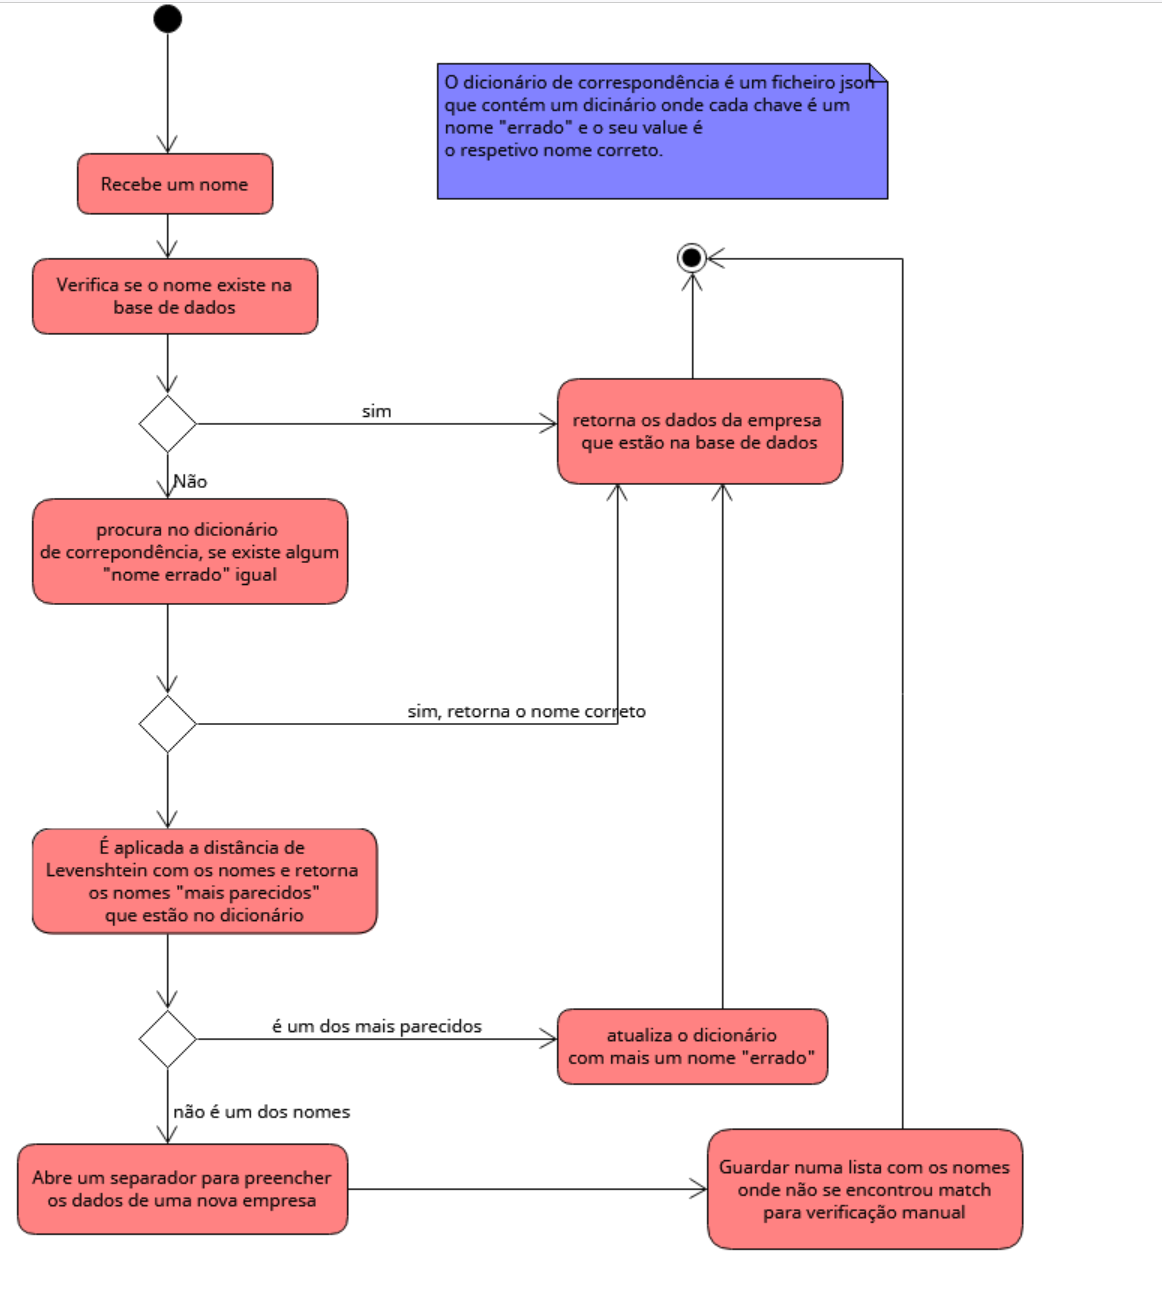
\includegraphics[width=0.8\textwidth]{images/system_design.png}
    \caption{Fluxo do Sistema de Correção de Nomes}
    \label{fig:design}
\end{figure}

\subsection{Soluções Alternativas}

Durante o desenvolvimento, outras soluções foram consideradas, cada uma com vantagens e desvantagens:

\begin{enumerate}
    \item \textbf{Uso de apenas a distância de Levenshtein}  
    \begin{itemize}
        \item \textbf{Vantagem}: Simplicidade na implementação, já que todas as entradas seriam corrigidas com base na proximidade.
        \item \textbf{Desvantagem}: Correções repetidas ou erros tipográficos frequentes poderiam causar inconsistências, já que não há memória de correções passadas, além disso o grau de incerteza seria maior.
    \end{itemize}
    
    \item \textbf{Uso de Machine learning}  
    \begin{itemize}
        \item \textbf{Vantagem}: Um modelo treinado poderia identificar padrões de erros mais complexos, aprendendo a corrigir mesmo entradas fora do comum.
        \item \textbf{Desvantagem}: Exige grande quantidade de dados e tempo para treinar o modelo. Além disso, não é ideal para aplicações onde a precisão manual e revisões humanas são mais adequadas, além disso o seu uso neste projeto seria desnecessário e excessivamente complexo, considerando a natureza do problema.
    \end{itemize}
    
    \item \textbf{Criação de um dicionário manual}  
    \begin{itemize}
        \item \textbf{Vantagem}: Total controlo sobre as correções.
        \item \textbf{Desvantagem}: Processo manual e inviável para grandes volumes de dados.
    \end{itemize}
\end{enumerate}

\subsection{Solução escolhida}

Em última análise, optou-se pela combinação do dicionário JSON com a métrica de distância de Levenshtein por diversos motivos:  
\begin{itemize}
    \item \textbf{Eficiência}: Correções rápidas para nomes já conhecidos, reduzindo a necessidade de cálculos repetidos.
    \item \textbf{Adaptabilidade}: O sistema está a ser melhorado continuamente à medida que novas associações são registadas no JSON.
    \item \textbf{Facilidade de revisão}: Entradas não resolvidas são organizadas para análise manual, garantindo precisão.
\end{itemize}

Esta abordagem equilibra eficiência automatizada e controlo manual, atendendo aos requisitos do projeto e garantindo um sistema flexível e preciso para validação de nomes.

% \section{Desenvolvimento atual}
% \subsection{Progresso}
% O projeto atualmente encontra-se na sua fase mais crucial e trabalhosa, tal como o nome do projeto sugere a mineração de texto incorpora um papel importante no desenvolvimento deste projeto, com o objetivo de conseguir criar um sistema para a standardização das bases de dados do Porto de Sines é importante que tenhamos a certeza de que os valores que estamos a utilizar para a standardização estão corretos, neste momento o projeto encontra-se numa fase em que estamos focados em fazer uma associação correta entre os dados corretos e os dados incorretos, para este fim estamos a utilizar uma técnica para cálculo de diferênças entre strings, a distância de Levenshtein, criada em 1965 por Vladimir Levenshtein. O nosso objetivo para o futuro seria com esta técnica conseguir criar um dicionário em que temos os nomes incorretos como chave e os nomes corretos como valor para consulta e correção eficiente dos dados.

% \subsection{Demonstração}
% A demonstração do nosso projeto é feita em python já que contem disponivéis várias bibliotecas que facilitam a manipulação de dados.
% Apesar de não demonstrar todas as capacidades que tencionamos que existam no final do projeto, já apresenta o fundamental.
% A demonstração foi feita num ambiente bastante controlado já que a quantidade de dados corretos que temos para utilizar é pequena.
% Lê o ficheiro onde está guardado o dicionário com os nomes incorretos associados aos nomes corretos.
% \vspace{0.5cm}

% 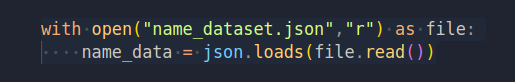
\includegraphics[width=14cm]{images/Screenshot1.png} \\[0.5cm]
% Por cada nome existente no dataset procura as linhas do dataset onde o nome é igual e também procura na tabela de dados standardizados a linha correspondente à correção desse nome.
% Se o nome não existir no dicionário de nomes é adicionado á lista de nomes desconhecidos.
% Se o nome existir no dicionário de nomes, substitiu todas as linhas com esse nome para os valores corretos presentes no dataset standard.
% \vspace{0.5cm}

% 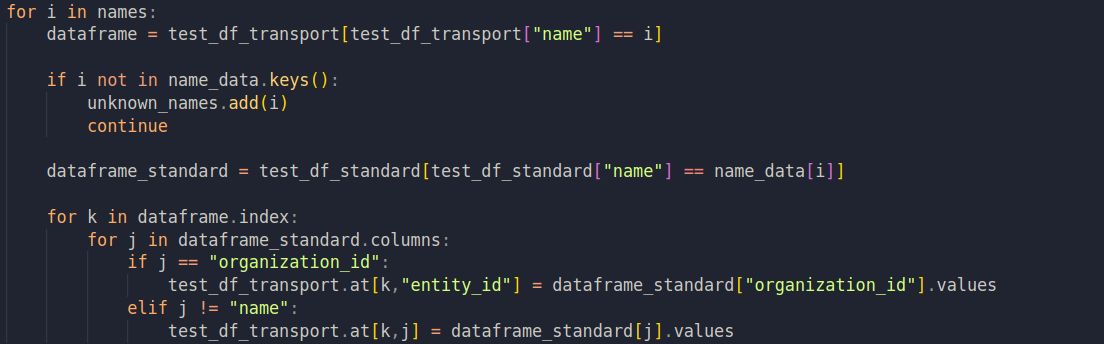
\includegraphics[width=14cm]{images/Screenshot2.png} \\[0.5cm]
% Para cada nome desconhecido devolve uma lista com os nomes standard mais próximos e pergunta ao utilizador se pretendia referir-se a algum deles. Se sim uma nova entrada é adicionada ao dicionário de nomes conhecidos.
% \vspace{0.5cm}

% 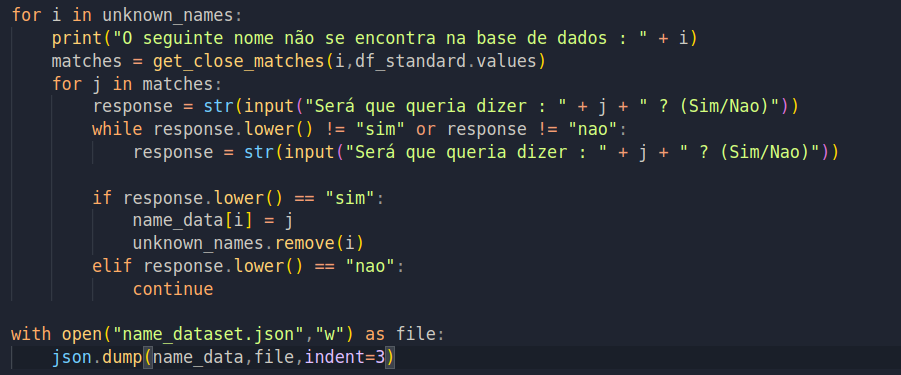
\includegraphics[width=14cm]{images/Screenshot3.png} \\[0.5cm]
% Se depois deste processo ainda existirem nomes desconhecidos é perguntado ao utilizador se pretende adicionar um novo nome á lista de nomes standard e ao dicionário de nomes, se sim então é lhe pedido que preêncha mais informações sobre o nome para que no futuro possam ser corrigidas linhas com esse nome.
% \vspace{0.5cm}

% 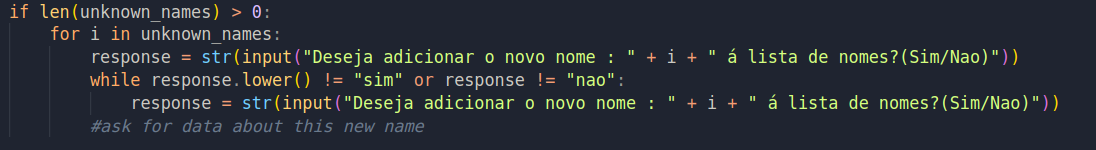
\includegraphics[width=14cm]{images/Screenshot4.png} \\[0.5cm]

% \subsection{Desafios e lições aprendidas}
% O maior desafio que estamos a enfrentar no momento centra-se precisamente no objectivo principal do projeto, a correção dos dados incorretos, devido ao tamanho dos dados fornecidos e á quantidade de erros cometidos nos mesmos o processo de associação dos nomes não pode ser feito manualmente já que demoraria imenso tempo, por isso como solução para este problema vamos utilizar métodos computacionais para determinar a correção de cada nome. 

% \newpage
% \bibliographystyle{plain}
% \bibliography{references}

\end{document}